\chapter{Preparation of Approach}
\label{ch:PrepApproach}
This chapter provides fundamental information about the techniques and notation used in the approach. As introduced in Chapter \ref{ch:CoCoME}, the Case Study's system specification is given in terms of detailed use cases. However, the proposed approach uses business processes as input. It is therefore necessary to provide a formal concept that assists with transforming use cases into business processes. \\
The following sections introduce a well known and established use case notation technique, a standardized notation to capture business processes and a structured approach to transform use case sets as business processes. Further, the extraction of data flow and control flow from business processes is discussed.








%TODO Nochmal drüber lesen kommt das in die DIscoussion?!


\section{Control Flow and Data Flow in BPMN Processes}
\label{ch:PrepApproach:ControlDataFlowBPMNProcess}
The approach uses structural and data object dependencies extracted from the control flow and data flow in order to build graphs, generate clusters and identify microservices. For this reason, the following sections explain how to extract these information from the given BPMN Processes. 

\subsection{Extract Control Flow of BPMN Processes}
Extracting the Control Flow in BPMN processes is a trivial task. The BPMN was originally designed to describe the control flow in business process. All that has to be done is to delete the Data Objects and the accompanying associations. The remaining diagram visualizes the control flow, including activities and their control flow dependencies. Further information, can be extracted in various ways. For instance, counting the amount of tasks between a pair of activities provides information about their structural dependency.

\subsection{Extract Data Flow of BPMN Processes}
First of all, data flows are usually represented using specific notations of Data Flow Diagrams (DFD), i.e. a notation proposed by E.Yourdon \cite{YourdonDFD}. For simplicity's sake, we relinquish to introduce another model notation and use the BPMN symbols instead. \\
As previously described, BPMN is only capable to express the data needs and the data results of single activities, whereas the data flow describes the flow of data in a process. By way of Fig.\ref{fig:restoreDataFlow}, \textit{Step 1} reads \textit{Data Object 1} and writes \textit{Data Object 2}. Despite the information about the data reads and writes of \textit{Step 1}, it is not possible to determine without further knowledge, if any information of \textit{Data Object 1} is used to write into \textit{Data Object 2}. Usually, this information has to be provided by system experts. \\
However, the approach presented in this thesis aims to reduce the required expertise or at least the additional information that is necessary when applying the approach. 
As a consequence, it is fundamental to approximate the data flow based on the data needs and writes of each activity. The approximation of the data flow works similar to the previous process. First of all, control flow related parts like sequence flows arcs, gateways, events and triggers are deleted. The remaining parts are tasks, data objects and data associations. Now, the tasks are not connected to their previous neighbours, with which they might exchange data, where the data exchange is synonymous with the flow of data.
To re-establish the possible data flow, follow the previously deleted control flow and reconnect the tasks with data association arcs by applying the following rules:


\begin{itemize}
	\item Connect a pair of tasks if previously connected by a control flow arc and 
	if another data object access happens in the course of the control flow (cf. Fig\ref{fig:restoreDataFlow})
	\item Replace gates by using two data association arcs (cf. Fig.\ref{fig:splitDataFlow} and Fig.\ref{fig:mergeDataFlow}). 
	\item Remove the remaining tasks that are not connected by data association arcs (cf. Fig.\ref{fig:removeDataFlow})
	
\end{itemize}
The remaining Graph contains all relevant tasks, the data objects and data associations that indicate the flow of data.

%"l, b, r, t"
\begin{figure}[h!]
	\centering
	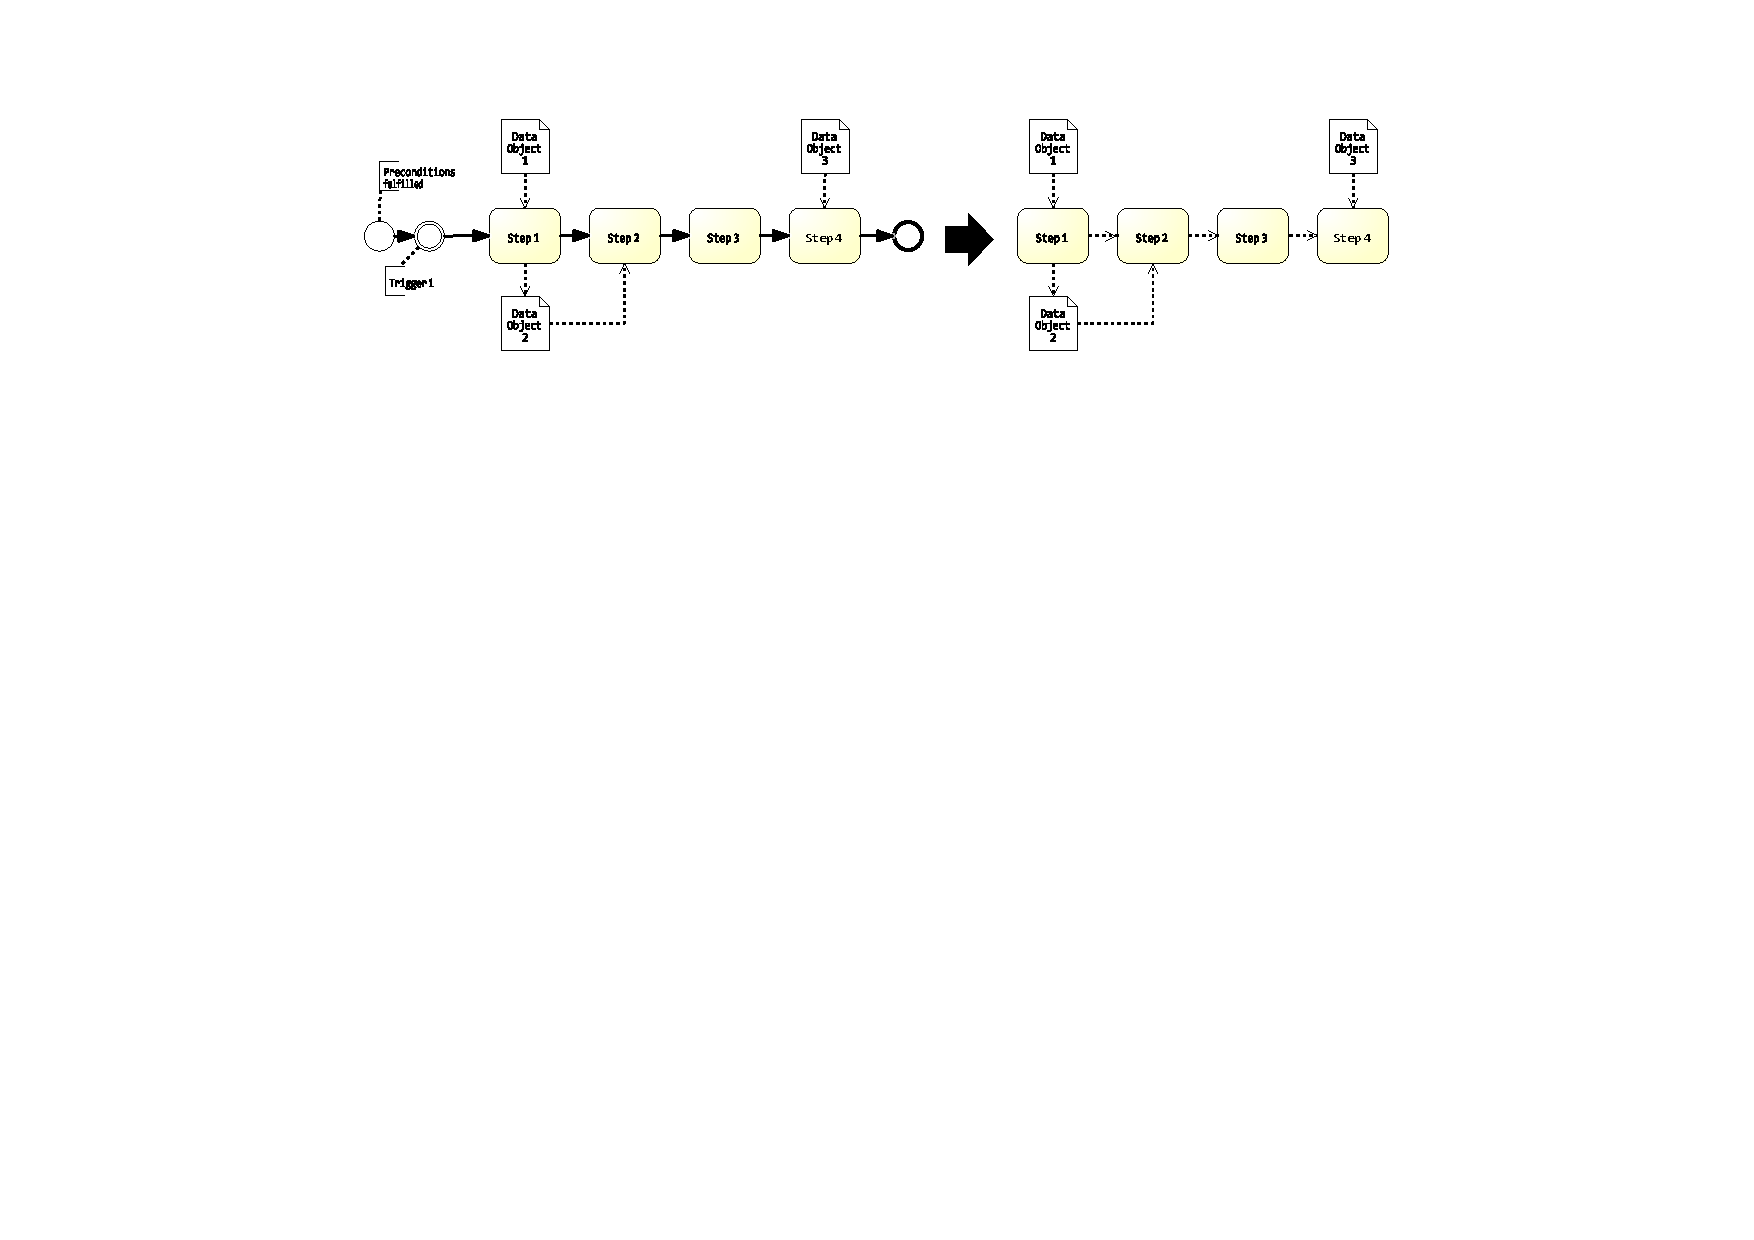
\includegraphics[width=\textwidth, trim={7.5cm 15cm 7cm 2cm}]{img/ExtractDFDRestore.pdf}
	\caption{Restore data flow connection}
	\label{fig:restoreDataFlow}
\end{figure}

\begin{figure}[h!]
	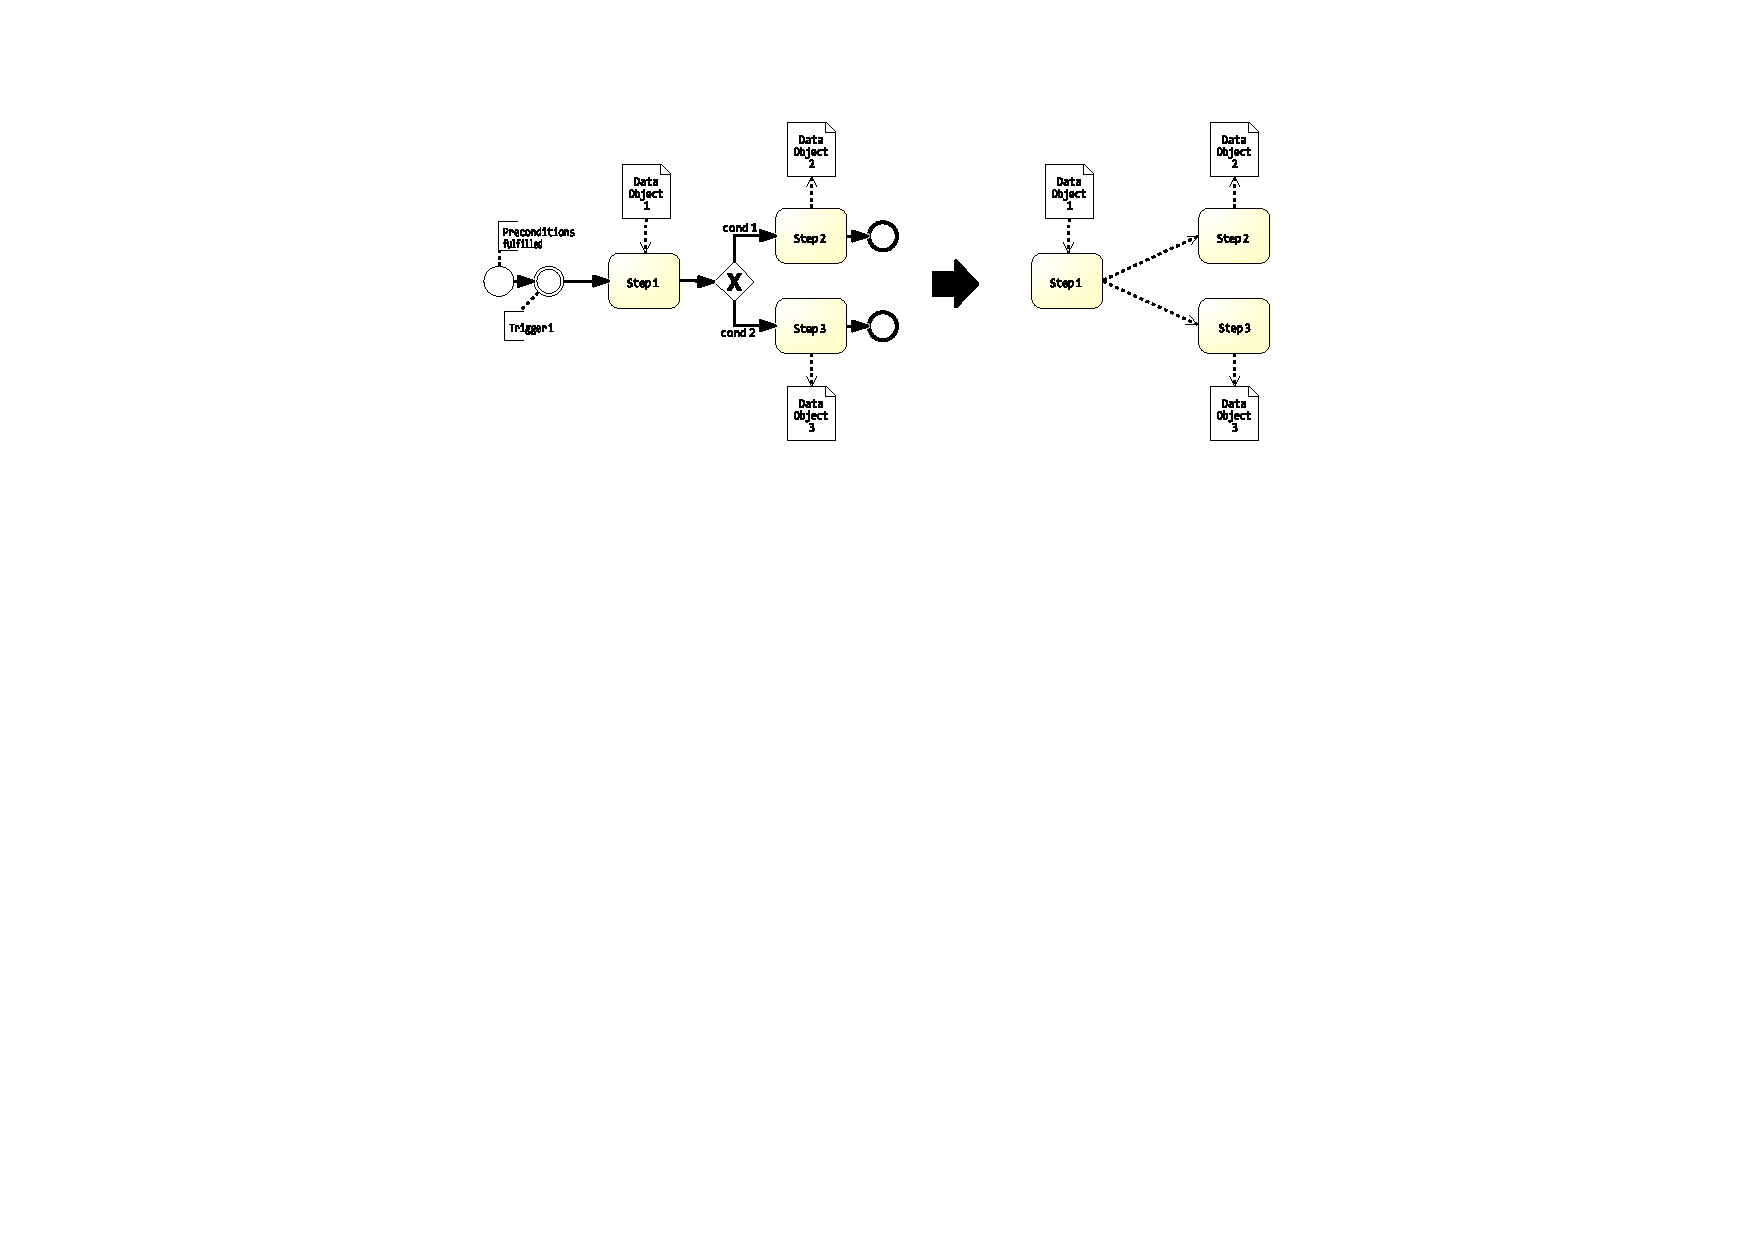
\includegraphics[width=14cm, trim={8.5cm 13.8cm 8.5cm 2.2cm}]{img/ExtractDFDGateWaySplit.pdf}
	\caption{Split data flow connection}
	\label{fig:splitDataFlow}
\end{figure}

\begin{figure}[h!]
	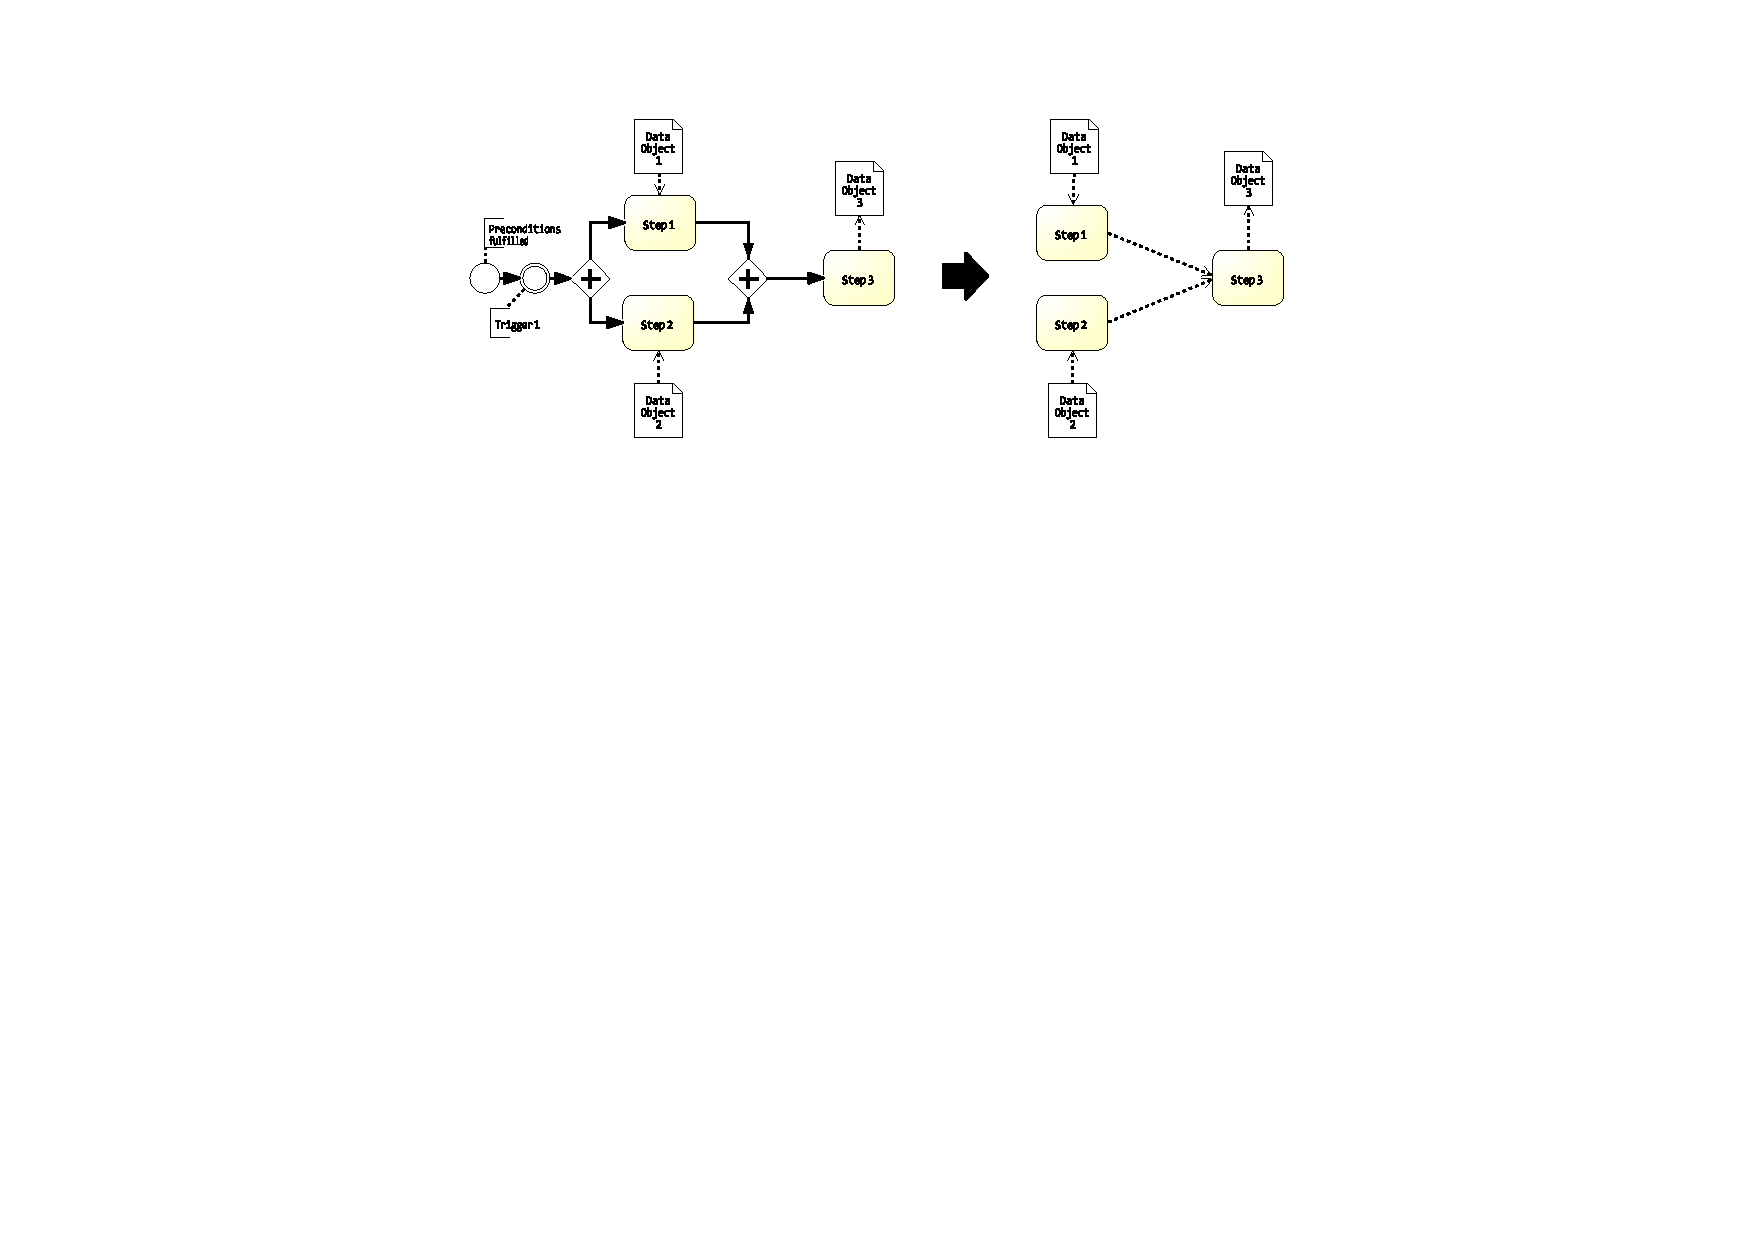
\includegraphics[width=14cm, trim={8.5cm 13.5cm 8.5cm 2.0cm}]{img/ExtractDFDGateWayMerge.pdf}
	\caption{Merge data flow connection}
	\label{fig:mergeDataFlow}
\end{figure}

\begin{figure}[h!]
	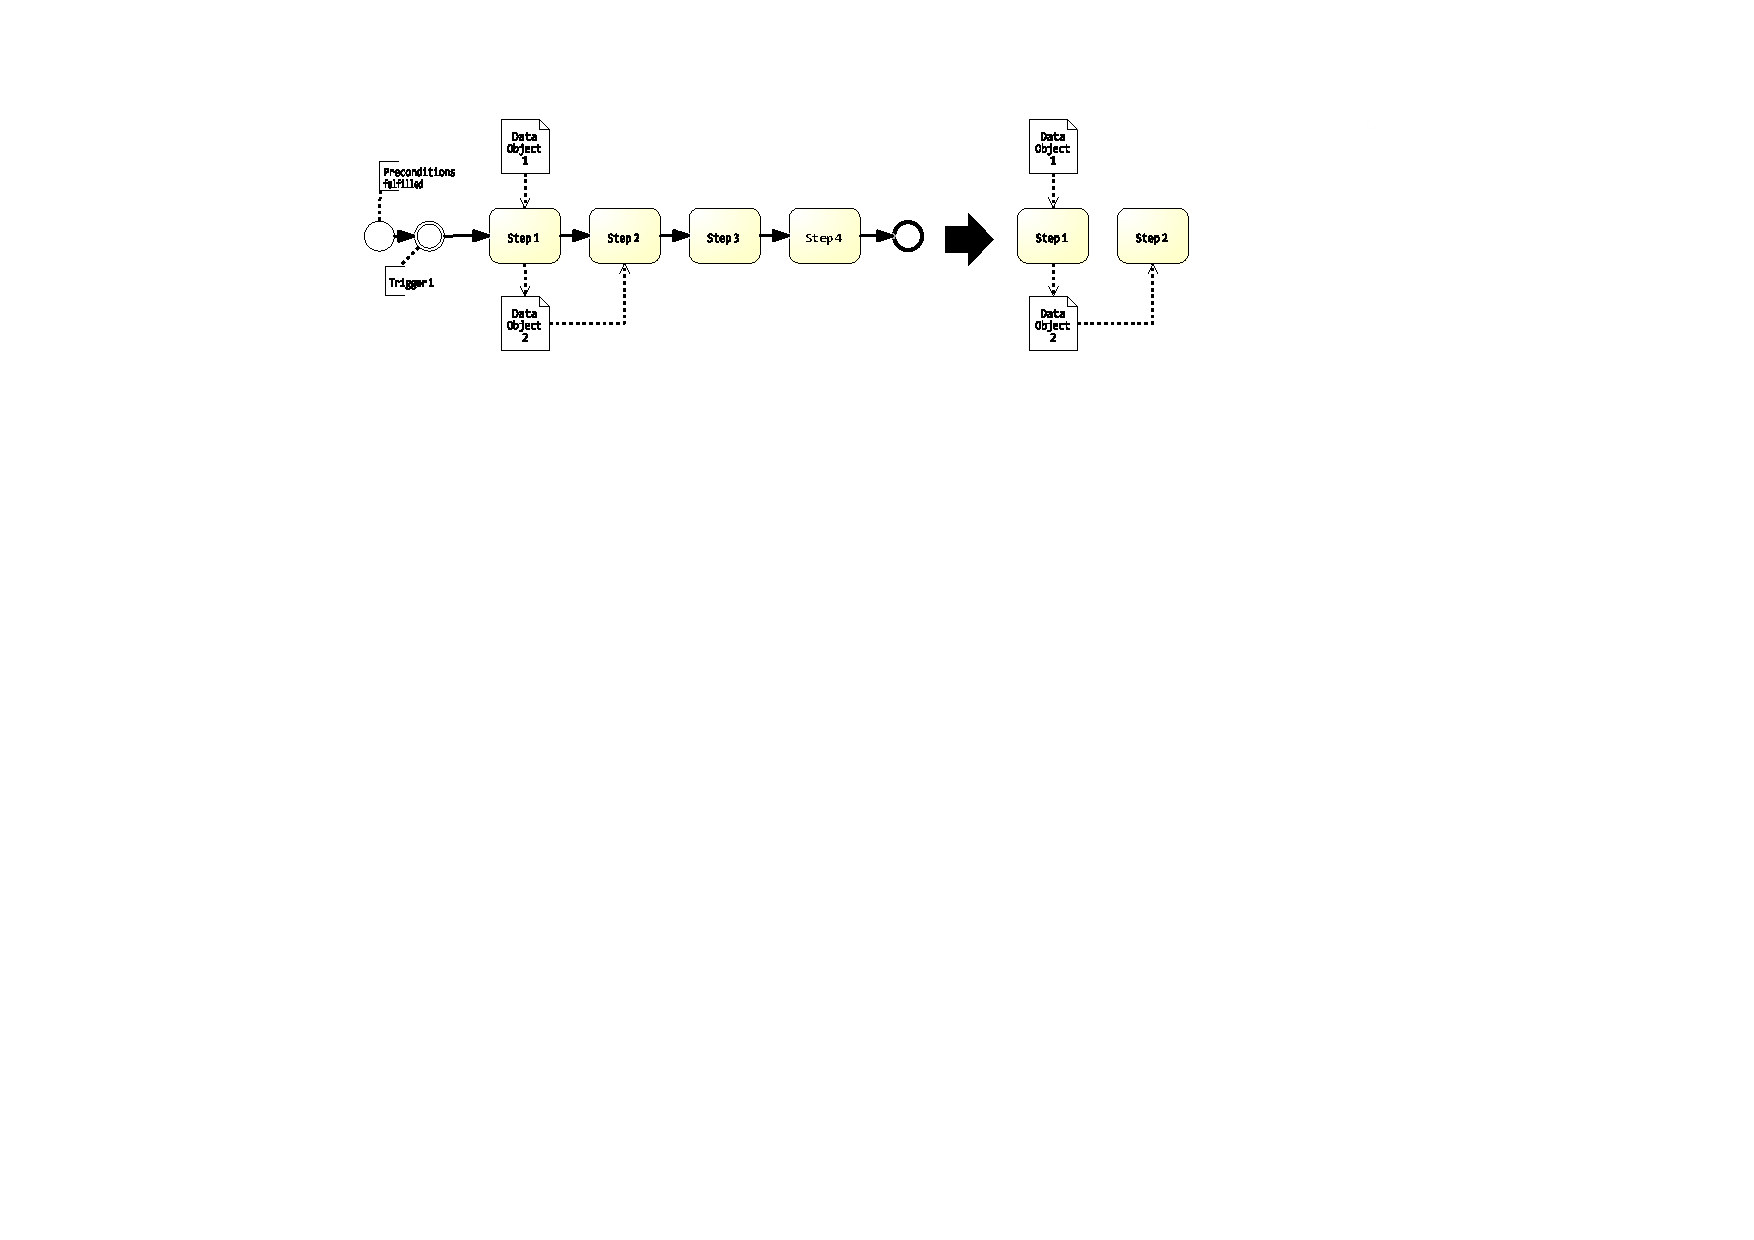
\includegraphics[width=\textwidth, trim={7.5cm 15.3cm 8.5cm 1.5cm}]{img/ExtractDFDRemove.pdf}
	\caption{Remove unnecessary tasks}
	\label{fig:removeDataFlow}
\end{figure}












